\documentclass[chi_draft]{sigchi}

% Use this section to set the ACM copyright statement (e.g. for
% preprints).  Consult the conference website for the camera-ready
% copyright statement.

% Copyright
%\CopyrightYear{2016}
%\setcopyright{acmcopyright}
%\setcopyright{acmlicensed}
%\setcopyright{rightsretained}
%\setcopyright{usgov}
%\setcopyright{usgovmixed}
%\setcopyright{cagov}
%\setcopyright{cagovmixed}
% DOI
%\doi{http://dx.doi.org/10.475/123_4}
% ISBN
%\isbn{123-4567-24-567/08/06}
%Conference
%\conferenceinfo{CHI'16,}{May 07--12, 2016, San Jose, CA, USA}
%Price
%\acmPrice{\$15.00}

% Use this command to override the default ACM copyright statement
% (e.g. for preprints).  Consult the conference website for the
% camera-ready copyright statement.

%% HOW TO OVERRIDE THE DEFAULT COPYRIGHT STRIP --
%% Please note you need to make sure the copy for your specific
%% license is used here!
% \toappear{
% Permission to make digital or hard copies of all or part of this work
% for personal or classroom use is granted without fee provided that
% copies are not made or distributed for profit or commercial advantage
% and that copies bear this notice and the full citation on the first
% page. Copyrights for components of this work owned by others than ACM
% must be honored. Abstracting with credit is permitted. To copy
% otherwise, or republish, to post on servers or to redistribute to
% lists, requires prior specific permission and/or a fee. Request
% permissions from \href{mailto:Permissions@acm.org}{Permissions@acm.org}. \\
% \emph{CHI '16},  May 07--12, 2016, San Jose, CA, USA \\
% ACM xxx-x-xxxx-xxxx-x/xx/xx\ldots \$15.00 \\
% DOI: \url{http://dx.doi.org/xx.xxxx/xxxxxxx.xxxxxxx}
% }

\toappear{}

% Arabic page numbers for submission.  Remove this line to eliminate
% page numbers for the camera ready copy
\pagenumbering{arabic}

% Load basic packages
\usepackage{balance}       % to better equalize the last page
\usepackage{graphics}      % for EPS, load graphicx instead 
\usepackage[T1]{fontenc}   % for umlauts and other diaeresis
\usepackage{txfonts}
\usepackage{mathptmx}
\usepackage[pdflang={en-US},pdftex]{hyperref}
\usepackage{color}
\usepackage{booktabs}
\usepackage{textcomp}

% Some optional stuff you might like/need.
\usepackage{microtype}      % Improved Tracking and Kerning
\usepackage[all]{hypcap}    % Fixes bug in hyperref caption linking
\usepackage{ccicons}        % Cite your images correctly!
\usepackage[utf8]{inputenc} % for a UTF8 editor only

% If you want to use todo notes, marginpars etc. during creation of
% your draft document, you have to enable the "chi_draft" option for
% the document class. To do this, change the very first line to:
% "\documentclass[chi_draft]{sigchi}". You can then place todo notes
% by using the "\todo{...}"  command. Make sure to disable the draft
% option again before submitting your final document.
\usepackage{todonotes}

% Paper metadata (use plain text, for PDF inclusion and later
% re-using, if desired).  Use \emtpyauthor when submitting for review
% so you remain anonymous.
\def\plaintitle{Improving legitimacy and efficiency of decisions in democratic communities}
%\def\plainauthor{First Author, Second Author, Third Author,
%  Fourth Author, Fifth Author, Sixth Author}
%\def\emptyauthor{}
%\def\plainkeywords{Authors' choice; of terms; separated; by
%  semicolons; include commas, within terms only; required.}
%\def\plaingeneralterms{Documentation, Standardization}

% llt: Define a global style for URLs, rather that the default one
\makeatletter
\def\url@leostyle{%
  \@ifundefined{selectfont}{
    \def\UrlFont{\sf}
  }{
    \def\UrlFont{\small\bf\ttfamily}
  }}
\makeatother
\urlstyle{leo}

% To make various LaTeX processors do the right thing with page size.
\def\pprw{8.5in}
\def\pprh{11in}
\special{papersize=\pprw,\pprh}
\setlength{\paperwidth}{\pprw}
\setlength{\paperheight}{\pprh}
\setlength{\pdfpagewidth}{\pprw}
\setlength{\pdfpageheight}{\pprh}

% Make sure hyperref comes last of your loaded packages, to give it a
% fighting chance of not being over-written, since its job is to
% redefine many LaTeX commands.
\definecolor{linkColor}{RGB}{6,125,233}
%\hypersetup{%
%  pdftitle={\plaintitle},
%% Use \plainauthor for final version.
%%  pdfauthor={\plainauthor},
%  pdfauthor={\emptyauthor},
%  pdfkeywords={\plainkeywords},
%  pdfdisplaydoctitle=true, % For Accessibility
%  bookmarksnumbered,
%  pdfstartview={FitH},
%  colorlinks,
%  citecolor=black,
%  filecolor=black,
%  linkcolor=black,
%  urlcolor=linkColor,
%  breaklinks=true,
%  hypertexnames=false
%}

% create a shortcut to typeset table headings
% \newcommand\tabhead[1]{\small\textbf{#1}}

\newcommand\secref[1]{section \textit{\nameref{#1}}}

%%% GLOSSARY %%%
%
% community = group which votes
% proposal = what you vote on
% decision = result of a vote, accepted or rejected proposal
%
%%% END GLOSSARY %%%

% End of preamble. Here it comes the document.
\begin{document}

\title{Improving legitimacy and efficiency \\ of decisions in democratic communities}

%\numberofauthors{3}
%\author{%
%  \alignauthor{Leave Authors Anonymous\\
%    \affaddr{for Submission}\\
%    \affaddr{City, Country}\\
%    \email{e-mail address}}\\
%  \alignauthor{Leave Authors Anonymous\\
%    \affaddr{for Submission}\\
%    \affaddr{City, Country}\\
%    \email{e-mail address}}\\
%  \alignauthor{Leave Authors Anonymous\\
%    \affaddr{for Submission}\\
%    \affaddr{City, Country}\\
%    \email{e-mail address}}\\
%}

\maketitle

\begin{abstract}
%The Achilles heel of many major democracies is the eternal need for sufficient engagement and attention from the community.
%While there have been major efforts towards increasing these attributes within the community, we explore a fundamentally
%different approach: For a fixed level of community attention, how can we optimize the allocation of this attention to
%maximize productivity?
%We propose a novel "statistical quorum", derived using first principles, as one metric the community can use to focus
%attention, in turn making the entire decision-making process dynamic.
%We developed an online system centered around this metric and tested it in a 140-person community that holds weekly
%councils over the course of 16 weeks.  We found that the community was able to use the online system to simultaneously
%improve the legitimacy and efficiency of their decision-making process.
\todo[inline]{TODO}
\end{abstract}

%\category{H.5.m.}{Information Interfaces and Presentation
%  (e.g. HCI)}{Miscellaneous} \category{See
%  \url{http://acm.org/about/class/1998/} for the full list of ACM
%  classifiers. This section is required.}{}{}
%
%\keywords{\plainkeywords}

\section{Introduction}

In many historical and recent elections it is not infrequent that we get close results.
Especially when this is combined with low voter turnout, how can we have confidence in results?
What if elections would be a day longer? What if they would be on a different day? What if
more people would participate? Would results still be the same?

An underlying question is what should we do when not everyone in the population votes.

Traditionally, we can have a stance that everyone had an opportunity to vote and express
their preference, so whatever are results based those who voted are legitimate results.
Research shows, though, that there are many reasons why people do not vote and that there
are many issues related to how elections are organized, i.e., are they held on working
or work-free day.

Alternatively, we can see voting as a survey and cast votes as a sample, although imperfect
and non-randomly selected, from a larger population, with a goal to infer the preference
of the whole population. In this setting we can use statistical methods to evaluate the
confidence we can have in the results.

Our contributions are as follows:

\begin{itemize}
\item We developed a framework of computing statistical credibility of results
based on sample size, votes cast, and voting duration.
\item Based on this framework we developed a concept of \emph{statistical quorum}
as a threshold of votes required to deem results legitimate.
\item We implemented an online application \emph{PeerMind},
integrating credibility of results and statistical quorum, and designed
a workflow of its use in a decision making processes.
\item We deployed the application in a democratically run community of 140
members for 5 months.
\item We show how use of statistical quorum improves utilization of collective
attention, increases overall participation, and increases number of decisions made
while not sacrificing their legitimacy.
\end{itemize}

\todo[inline]{Structure of the paper.}

%
%
%Many communities use voting to make collective decisions.
%\todo{Should we support this statement with a reference?}
%In its basic form, voting consists of members of a community casting a vote \emph{in favor} or \emph{against} a decision.
%If the majority ($> 50\%$) of votes are in favor of the decision, the decision \emph{passes} and is adopted as a decision
%of the whole community.
%
%There have been many improvements proposed to this basic form and various analysis made.
%\todo{Add references.}
%In this paper we focus on the question of \emph{quorum} and how high the quorum should be.
%Quorum is the minimum number of members participating in voting for voting to be seen as representative of the whole
%community, i.e., legitimate.
%If quorum is too low, decisions adopted might not represent the community.
%If it is too high, the community might have issues achieving the quorum.
%Not enough members might decide to participate in voting, or members might on purpose boycott voting to
%prevent decision to be adopted, even if those opposing it are in minority.
%Communities often decide quorum arbitrarily\footnote{Robert's Rules of Order states that the quorum
%``should approximate the largest number that can be depended on to attend any meeting except in very bad weather
%or other extremely unfavorable conditions.''~\cite{roberts}}
%and try to increase participation of members in communities' democratic processes through various means
%to address the issue of too low turnout.
%\todo{Add references. Mention forced participation in some countries.}
%Moreover, many democratic communities have issues achieving quorum which hinders their operation.
%\todo{Add references.}
%
%Even if voting turnout has reached legally required quorum, or when one is not defined,
%it is still a question how to evaluate if the turnout is high enough to find results legitimate.
%As an example we can look at two recent votes, Brexit, a 2016 referendum for United Kingdom's withdrawal
%from the European Union, and popular vote in 2016 USA presidential elections, as seen in Table~\ref{tab:example}.
%Ignoring particularities of USA presidential elections process and using a popular vote as an example,
%how can we reason about legitimacy of results?
%
%\begin{table*}
%  \centering
%  \begin{tabular}{l r r r r r r r}
%    {\small\textit{Vote}} & \multicolumn{2}{r}{\small \textit{First option}} & \multicolumn{2}{r}{\small \textit{Second option}} & {\small \textit{Total eligible voters}} & {\small \textit{Turnout}} & {\small \textit{Decision credibility}} \\
%    \midrule
%    Brexit & 17,410,742 & $51.9\%$ & 16,141,241 & $48.1\%$ & 46,500,001 & $72.2\%$ & $59.8\%$ \\
%    Presidential elections & 62,984,825 & $48.9\%$ & 65,853,516 & $51.1\%$ & 230,585,915 & $55.9\%$ & $52.6\%$ \\
%  \end{tabular}
%  \caption{Votes cast in Brexit, a 2016 referendum for United Kingdom's withdrawal from the European Union~\protect\cite{brexitresults},
%  and 2016 USA presidential elections, popular vote~\protect\cite{usaresults1,usaresults2}. Simplified to only two options and without
%  invalid votes. The last column shows computed decision credibility as described in \secref{sec:decision-credibility}. We see that
%  credibility is low, which we can mostly attribute to the fact that there is small difference in votes between both options so
%  with more votes any option could end up winning.}\label{tab:example}
%\end{table*}
%
%To answer this question we are proposing a novel metric, \emph{decision credibility}, which uses statistical
%hypothesis testing to evaluate the credibility of the voting result.
%It uses the distribution of votes made to evaluate the probability of a decision passing if everyone actually voted,
%and not just those who did vote.
%Intuitively, if, in a community of 100 members, 40 members vote for a decision to pass and nobody against,
%we can see that if everyone voted, the probability of majority of population voting for a decision is high.
%On the other hand, if 41 members for in favor and 40 against, we cannot really say much about what would a decision
%be if everyone voted.
%Only two more votes against can completely change the outcome.
%Hence, the suggested action would be for the community to gather more votes and continue discussion around the decision.
%We describe decision credibility in more detail in \secref{sec:decision-credibility}.
%
%Based on decision credibility we can define a \emph{statistical quorum} as a threshold which a decision's credibility
%has to pass for a decision to be seen as legitimate.
%For example, if we adopt $90\%$ as a reasonable requirement for statistical quorum and we compute decision
%credibility for votes in Table~\ref{tab:example} we see that in both cases we do not reach statistical quorum
%which puts legitimacy of those decisions into a question.
%We discuss a way for a community to determine a reasonable statistical quorum in \secref{sec:discussion}.
%
%Traditionally it is argued that legitimacy comes from the fact that members had a chance to participate
%and they decided not to, giving legitimacy to make a decision to those who did participate.
%We argue that this is a problematic view because there are many restrictions on why members could not
%participate and vote.
%For example, they might not had time to participate because of other commitments, or motivation, or they might determined
%that they are not informed enough to participate.
%Moreover, members are from different reasons in their communities and potentially contribute in other ways
%than by participating in its democratic processes.
%Instead of assuming that everyone could participate if they would want, or trying to increase participation,
%we can see amount of participation members are able to do as a limited resource, a \emph{collective attention}
%a community has available to utilize for its decision making.
%
%We can compute decision credibility during ongoing voting process to give feedback to the community
%on how contentious a proposed decision is how much more votes are necessary for a statistical quorum
%to be reached.
%This allows the community to focus its collective attention towards decisions which require more votes
%to determine a legitimate result, while reducing attention towards proposals which already have overwhelming support.
%Instead of trying to increase participation on all democratic decisions being made, a community can
%do that selectively through an automatic feedback loop, trying to reach statistical quorum for their decisions.
%
%We built an open source web application PeerMind integrating statistical quorum with online voting.
%The application exposes computed decision credibility to users in real-time and through that provides
%the feedback loop needed for improving utilization of collective attention.
%We present the application in \secref{sec:peermind} and use it for evaluating statistical quorum in
%\secref{sec:evaluation}.
%
%\todo[inline]{Should we explicitly list our contributions again?}
%
%\todo[inline]{Repeat the structure of the rest of the paper? Is there a better way to reference sections than
%referencing it by name?}

\section{Related Work}

%\todo[inline]{Repeat references from "There have been many improvements proposed to this basic form and various analysis made."?}
%
%\todo[inline]{Threshold and quorum at \url{https://www.publications.parliament.uk/pa/ld200910/ldselect/ldconst/99/99.pdf}.
%How do some claim that quorum are in fact bad, and counter democratic, but do not offer a solution how to evaluate decisions.}
%
%\todo[inline]{Voting auditing work.}
%
%\todo[inline]{Delegation as way to increase legitimacy, Liquid Democracy, etc.}
%
%\section{PeerMind Web Application}
%\label{sec:peermind}
%
%\todo[inline]{Something we need to think about is the level of detail we want to go into regarding the implementation/features of PeerMind beyond statistical quorum and range voting.  I think we might want to focus on only those two features for this paper.\\
%I think PeerMind as a comprehensive platform should have its own paper where all of the data is analyzed across the board.  This would be a much more typical HCI paper.  (If I can become president of Ridge in a future semester, we'll have another chance to run a clean, well-designed experiment with a much more developed version of PeerMind.)\\
%The message in the current paper might be clearest if we keep the scope focused on the theory + evaluation/verification.  We should make sure we're not trying to pack too much into one paper.
%\\---Max}
%
%We built a full-fletched real-time web application for collective decision making and voting using Meteor
%framework~\cite{meteor}.
%Users can initiate new discussions which leads them to the main user interface for each discussion as seen
%in Figure~\ref{fig:peermind}.
%
%\begin{figure*}
%  \centering
%  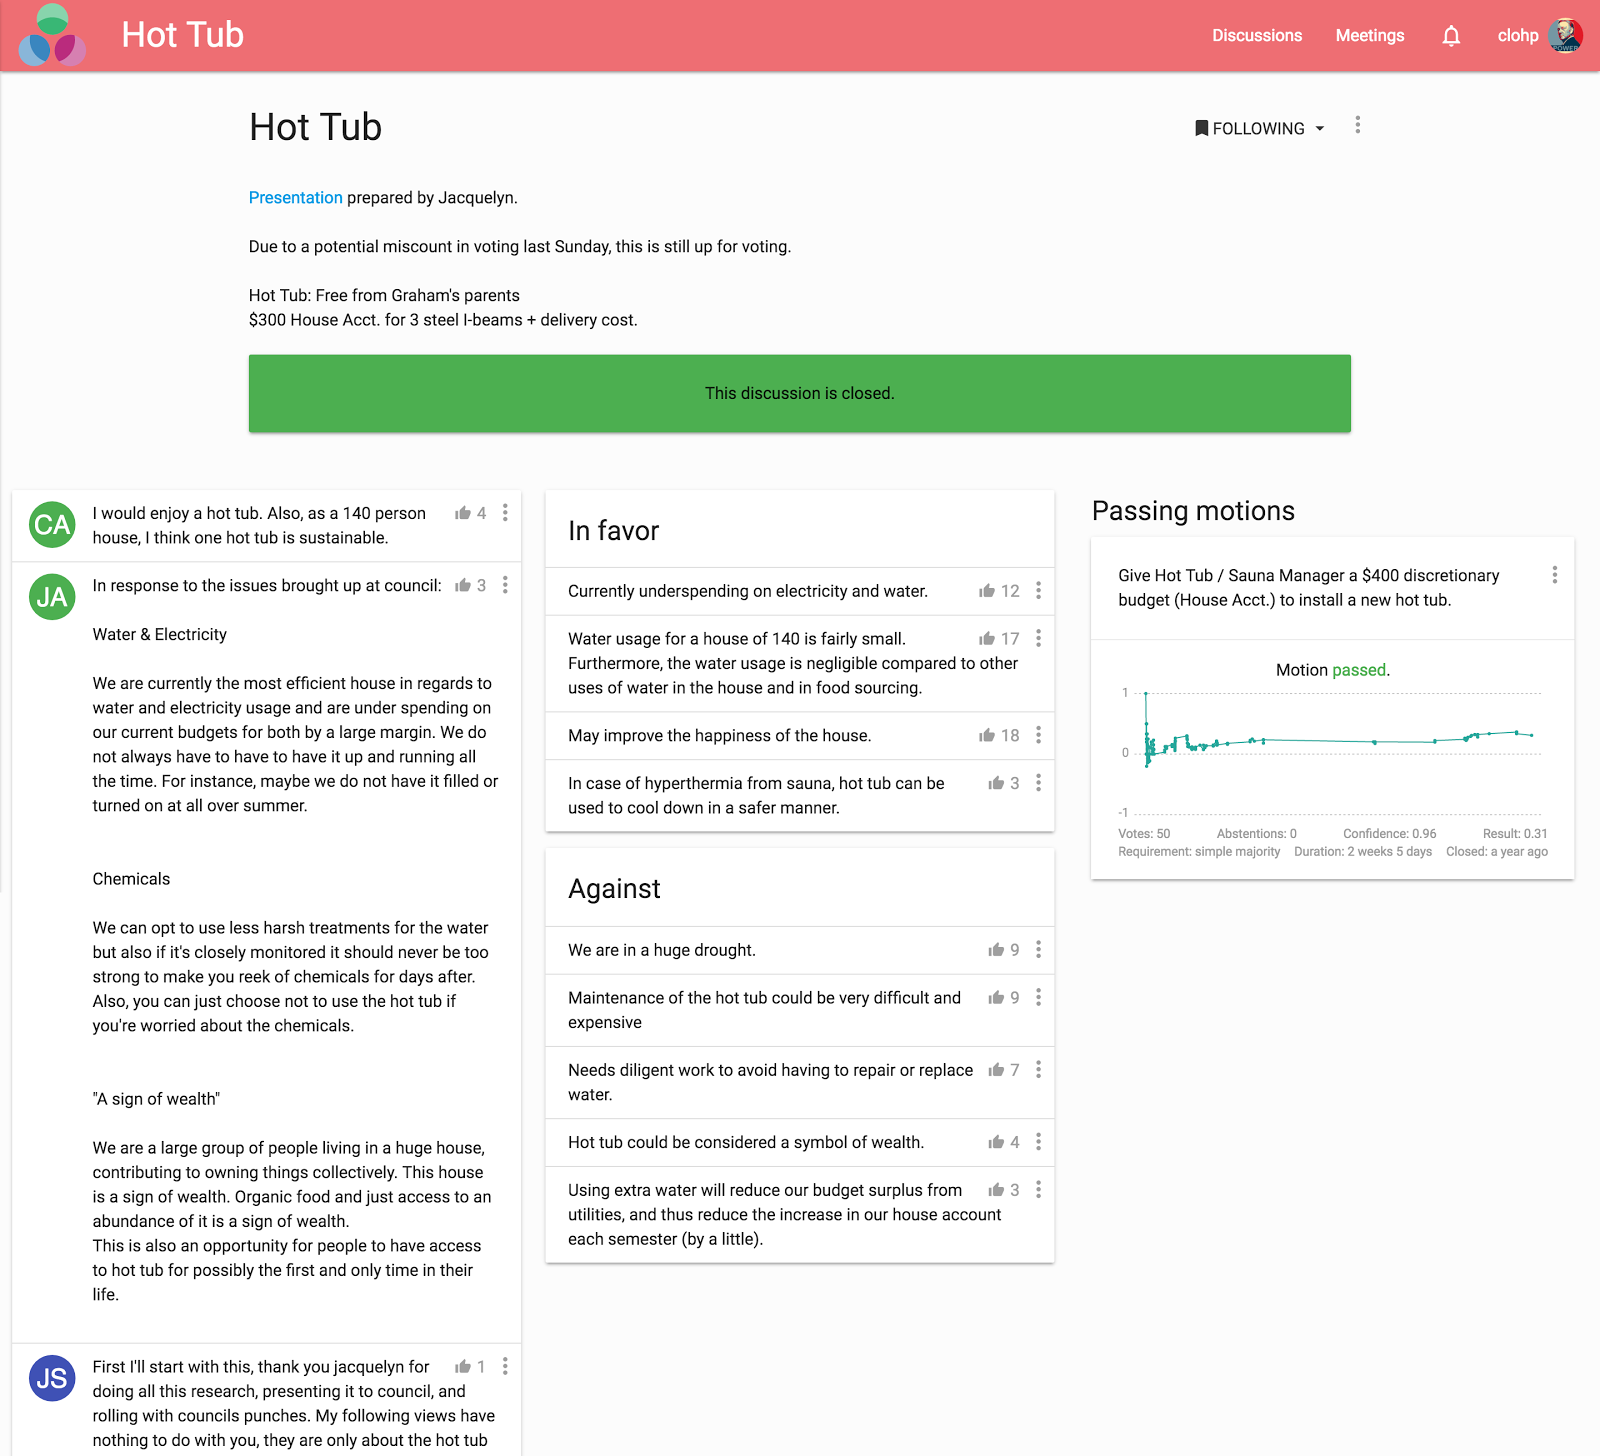
\includegraphics[width=1.75\columnwidth]{figures/peermind.png}
%  \caption{The main PeerMind interface of a discussion. There is initial discussion description on the top and under it there
%  are three columns. A commenting sections for users to discuss it and proposed decisions, a second column where moderators can
%  summarize arguments made during discussion, and a list of proposals to address the discussion.
%  Proposals can be in different states: a proposal being discussed, a proposal being voted on, and with voting concluded.}\label{fig:peermind}
%\end{figure*}
%
%%and discuss them with others online in real-time and with rich-text content.
%%They can attach images and files using drag\&drop. Moderators can summarize discussions into three groups
%
%\todo[inline]{Present how users can see ongoing results during voting. Show an image of active ballot, but with expanded view for current results.}
%
%%Range voting (also known as score voting) is voting where members of a community express their positions on open proposals by assigning
%%each a score on a fixed scale, in the context of this paper, between $-1$ and $+1$.
%%A proposal passes if the average score of all votes on a position is positive.
%%When multiple competing proposals are being voted on, the one with highest average score wins.
%%
%%Prior work has shown that this approach generalizes many previous approaches to voting and allows members to express their
%%positions in a highly informative and precise manner.
%%We find it especially suitable for a web application because many web users are used to use it when ranking products
%%and giving other ``five-star'' feedback.
%%Moreover, if later on a new proposal is added to a set of existing proposals on which voting was already open, only the
%%new proposal needs to be evaluated by members, as opposed to alternative voting systems where the relative rankings of
%%each proposal would need reassessing (assuming members use a consistent personal scale when voting).
%
%\todo[inline]{The app has features both for use in online and offline setting. This allows one to compute
%statistical quorum also for an in-person meeting because math is now more complicated than just counting hands.
%We focus on online experience in this paper.}
%
%\todo[inline]{Security is out of the scope of this work. We assume here that users and their identities are known and are managed
%by a community's admin. There are many communities where their decision making is public with public minutes and this is who
%the app is currently targeting.}

\section{Decision Credibility}
\label{sec:decision-credibility}
A statistical quorum uses statistical hypothesis testing to infer the credibility of the outcome of an open vote before the community adopts the outcome as being truly representative all members' positions.
For example, in a community of 100 members, if 35 members support a specific proposal and 0 oppose, then we can conclude with high probability that, had all 100 members taken the time to vote, a majority of them would be in support of the proposal.  Hence, despite the reality of 65 members not having voted, the outcome of the 35-member vote was credible enough to be taken as representative of the entire community's desire.
On the other hand, if 80 members vote, where 41 support the proposal and 39 oppose, then we cannot yet conclude that the decision to accept the proposal is credible enough for the entire community to officially adopt, despite the significant participation in the vote.
Instead, the suggested course of action would be to continue gathering more votes and/or further discussing the proposal until a credible outcome is established.

By utilizing a statistical quorum, a community can actively direct attention and participation within the community towards contentious proposals, while avoiding wasting attention on noncontroversial proposals.

\subsection{Background}
Consider a community that needs to collectively decide which proposal (if any) to accept out of a set of competing proposals.
To act in democratic fashion, the community may wish to select a winning proposal that either has the support of a \{simple, super\}-majority of all members, or instead is demonstrably preferred over all other competing proposals.  (In some cases, the community may want a winning proposal to satisfy both criteria.)

Ideally, we do not want to poll all members in order to officially accept a proposal, but we do want some level of certainty (e.g., $90\%$ certainty) that
the population is not accidentally accepting an undesired proposal, which in this case encompasses accepting a proposal that is not supported by a majority of members and/or is not clearly preferred over all other competing alternatives.

The primary motivation behind using a statistical quorum is to guarantee a level of credibility before letting a subset of members act on behalf of the entire community.

\subsection{Problem Statement}
We wish to compute the probability that the bias in a community towards supporting a proposal is greater than some
fraction of the population (e.g., $50\%$ for a simple majority, $67\%$ for a super majority).

In addition, we wish to compute the probability that the community bias towards supporting a specific proposal is greater than the community bias towards supporting any competing proposals.

\subsection{Assumptions}
We assume that there is a fixed latent bias for the support of a proposal within the community.  We take each individual vote to be independent and identically distributed (i.i.d.) according to a Bernoulli distribution around this bias.  It should be noted that the independence assumption may not hold in some settings, such as when votes are accumulated over time (one may observe surges of correlated votes).  We will partially address this when refining our original formulation of a statistical quorum into a \textit{dynamic} statistical quorum.

Without having collected any votes, we assume that the community bias may be any value between $0\%$ and $100\%$ with equal probability (uniform prior).

\subsection{Voting}
We allow for range voting where each member of the community may choose any real-valued vote $v \in [-1,+1]$ to
represent their vote, with $v = -1$ representing full opposition and $v=+1$ representing full support.  In most applications, it is sensible to quantize $v$ into a fixed number of bins spanning the full range, hence our treatment of $v$ as a discrete random variable.  Because we treat individual votes as a Bernoulli random variable, one can consider $v$ as an individual's average vote.  In the theory subsection below, we rescale $v$ to be in the range $[0,1]$ via the notation $\frac{v + 1}{2}$.

We allow voters to ``abstain'' from voting.
We treat abstentions as indicating that a voter is removing themselves from the community on a given vote.
It is important to distinguish an ``abstention'' (removing one's self from the voting population) from voting $0$ (indicating indifference).

\subsection{Bayesian Theory}

\todo[inline]{Weave in a single concrete example to ground all the abstract theory so that the entire derivation and motivation has a clear and cohesive thread from start to finish.}

After collecting an initial set of votes from members, we want to use that data to construct a prior distribution to help estimate the posterior probability that the proposal is acceptable to the entire community.  Because the sum of  the collected votes follows a binomial distribution, a commonplace and convenient choice for the form of the prior on the community's bias is the Beta distribution (due to its conjugacy with the binomial distribution).  Together, they form the Beta-binomial distribution (related to the P\'olya urn model).

After extracting the sufficient statistics from raw votes --- namely, the average score and the number of abstentions --- we can adjust the effective community size and corresponding threshold.  In addition, we can calculate the effective number of ``yes'' ($+1$) and ``no'' ($-1$) votes:

Let
\begin{description}
\begin{itemize}
\item[$C = $] $\{X_1,\ldots, X_n\}$, the set of competing proposals,
\item[$N = $] population size,
\item[$X_i = $] $\{v_1, \ldots, v_{m_i}\}$, the $m_i$ raw votes for proposal $i$, after excluding abstentions,
\item[$N_i = $] $(N - \textrm{number of abstentions on } X_i)$, the effective population voting on proposal $X_i$,
\item[$\alpha_i = $] $\sum\limits_{v \in X_i}\left(\frac{v+1}{2}\right)$, the effective number of ``yes'' votes on motion $X_i$,
\item[$\beta_i = $] $m_i - \alpha_i$, the effective number of ``no'' votes on motion $X_i$,
\item[$K_i = $] $N_i - m_i$, the number of remaining votes yet to be cast on $X_i$,
\item[$p_i = $] true latent community bias towards voting ``yes'' on $X_i$.
\end{itemize}
\end{description}

In Eqs. \eqref{eq2}, \eqref{eq3}, \eqref{eq5}, \eqref{eq6}, \eqref{eq7} that follow, we refer the reader to the \hyperref[sec:derivation]{Appendix} for complete derivation details and justifications.

When considering a single proposal $X_i$ in isolation, we wish to compute:
\begin{align}\label{eq1}
\Pr(\alpha^*_i > T_i \mid X_i),
\end{align}
where
\begin{description}
\begin{itemize}
\item[$\alpha^*_i = $] the total number of ``yes'' votes for $X_i$ if we were to sample the entire population,
\item[$T_i = $] $f \cdot N_i$, for some fraction $f$ corresponding to the type of majority needed for the vote
(e.g., $f=\frac{1}{2}$ for a simple majority).
\end{itemize}
\end{description}
Using a desirable prior 
\begin{align}\label{eq2}
p_i \mid X_i \sim \operatorname{Beta}(1+\frac{\alpha_i}{K_i},1+\frac{\beta_i}{K_i}),
\end{align}
corresponding to a uniform prior when no votes have been cast ($\alpha_i = \beta_i = 0$), we can express \eqref{eq1} as:
\begin{align}\label{eq3}
\Pr(\alpha^*_i > T_i \mid X_i) &= 1 - {CDF}_{\nu_i}(V_i)
\end{align}
for
\begin{align*}
&\nu_i \sim \operatorname{Beta-Binomial}(1 + \frac{\alpha_i}{K_i}c, 1 + \frac{\beta_i}{K_i}c, K_i),\\
&{CDF}_{\nu_i}(V_i)  = \Pr(\nu_i \leq V_i),
\end{align*}
\todo[inline]{Note that we choose $c=10$ because it leads to intuitive results.}
where
\begin{description}
\begin{itemize}
\item[$V_i = $] $\lfloor{T_i - \alpha_i}\rfloor$, the maximum number of additional ``yes'' votes $X_i$ could receive such that it would remain below threshold.
\end{itemize}
\end{description}

When considering a proposal $X_i$ relative to other proposals in $C$, we wish to compute
\begin{align}\label{eq4}
\Pr\left(\bigwedge_{j \neq i} (\alpha^*_i > \alpha^*_j) \mid C\right)
\end{align}

Under the assumption that the community's votes on motions are independent across motions (which, in many instances, will actually give a lower bound on \eqref{eq3} when a community's support of one proposal is negatively correlated with its support on a competing proposal), we can decompose \eqref{eq3} as follows:
\begin{align}\label{eq5}
& \Pr\left(\bigwedge_{j \neq i} (\alpha^*_i > \alpha^*_j) \mid C\right) \nonumber \\
= & \prod_{j \neq i}\left(1 - \sum_{k=\lceil\delta_{ij}\rceil}^{K_j} \Pr(\nu_j = k) \cdot {CDF}_{\nu_i}(\alpha_j + k) \right)
\end{align}
where
\begin{description}
\begin{itemize}
\item[$\delta_{ij} = $] $\alpha_i - \alpha_j$, the number of effective ``yes'' votes $X_i$ leads $X_j$ by.
\end{itemize}
\end{description}

Using Eqs. \eqref{eq2} and \eqref{eq4}, we can numerically compute the credibility of a vote's outcome in two key scenarios relevant for democratic communities.  For example, a community may only consider accepting a proposal when a vote's credibility is above $90\%$.

\subsection{Dynamic Statistical Quorum}
Oftentimes, not all proposals are relevant to the entire community.  Instead, a niche proposal may only affect a subset of the community, and hence to require much of the community to indicate their indifference and/or decide their opinion is a waste of the their fixed attentional budget.  While the underlying formulation for a statistical quorum was to establish credibility guarantees before taking action, a natural consequence in common scenarios of the kind just described leads to a reduction in decision-making efficiency.  How can we maintain credibility guarantees while simultaneously boosting efficiency?

The solution is to infer the \textit{relevant} population size that cares about a given proposal so that we may establish credibility within only the subset population (naturally requiring less global attention).  By replacing the absolute upper bound on this relevant population size ($N_i$) with a high probability upper bound, we can continue to use the same formula presented in Eqs. \eqref{eq2} and \eqref{eq4}, but with more relevant parameters (namely, a smaller $N_i$, which in turn modifies $T_i$, $K_i$, and $V_i$).

To infer $N_i$, we turn to a dynamic voting process whereby information embedded within the dynamics is exploited.  By modeling the arrival rate of new votes as a nonhomogeneous Poisson process, we can extrapolate into the future.  For a decaying arrival rate of new votes, a nonhomogeneous Poisson process $\{N(t),t\geq 0\}$ probabilistically models the number of future arrivals over a given time interval $[0,t)$ according to:
\begin{align*}
\Pr(N(t)=n)={\frac {[\Lambda (t)]^{n}}{n!}}e^{-\Lambda (t)},
\end{align*}
where
\begin{align*}
\Lambda (t)=\int _{0}^{t}\lambda (\tilde{t})\mathrm{d}\tilde{t},
\end{align*}
for some arrival rate process $\lambda (t)$.

For our purposes, we make a natural choice,
\begin{align}\label{eq6}
\lambda (t) = \lambda_0 {(\gamma)}^{\frac{t}{K_i/N_i}},
\end{align}
where
\begin{description}
\begin{itemize}
\item[$\lambda_0 =$] a time-averaged rate of vote arrivals (preferably over a unit of time that sufficiently smooths the historical rate),
\item[$\gamma =$] a decay factor ($0 < \gamma < 1$) ideally tuned to fit real historical data for the community via a regression analysis.
\end{itemize}
\end{description}
Now, for example, to upper bound with $95\%$ probability the remaining number of votes still pending, we wish to solve for $\hat{K_i}$ such that the following inequality is satisfied:
\begin{align}\label{eq7}
\lim_{t\rightarrow \infty}\Pr\left(N(t)\leq \hat{K_i}\right) & = \sum_{n=0}^{\hat{K_i}} \frac{\Lambda^n}{n!}e^{-\Lambda} \geq 95\%,
\end{align}
where $\Lambda = \frac{\lambda_0 \cdot K_i/N_i)}{\ln{1/\gamma}}$.
Upon solving for $\hat{K_i}$, we update $N_i \leftarrow \min\{N_i,\alpha_i + \beta_i + \hat{K_i}\}$, and can proceed to check for a statistical quorum using Eq. \ref{eq5}.


%\begin{figure}[ht]
%\centering
%\includegraphics[width=0.5\textwidth]{figures/}
%\caption{Simple Majority: $\alpha$ vs. $\Pr(\alpha > \frac{1}{2}N)$ for $N=100$, $\beta = 10$.}
%\label{simple_majority}
%\end{figure}

\section{Evaluation}
\label{sec:evaluation}

We evaluate statistical quorum in two ways. First, we evaluate it theoretically and explore its mathematical properties.
Then we evaluate it through real-world use of the PeerMind application by a 140 members community.

\subsection{Theory}

\todo[inline]{Visualize the credibility and dynamics of the voting process under this framework:\\
4 Figures and 1 Table Pending}

\subsection{Use in Existing Democratic Community}

\todo[inline]{See my comment at the beginning of the PeerMind Web App section.  I think the evaluation you note below about the interviews is out of the scope of this paper, which should be focused on statistical quorum and less online vs. offline platforms.\\
---Max}

\todo[inline]{Explain how we were using this for 16 weeks in fall 2016 in a community where traditionally they have
been meeting weekly and now they used it online. How X proposals have been made with Y votes.}

\todo[inline]{Explain how we compare with history: using minutes from spring 2016 for the same community. Issues with
quorum often not bein reached or being lost during the meeting. How many proposals were made then.}

\todo[inline]{Using our metric compare legitimacy of decisions being made in the spring and fall.}

\todo[inline]{We compare how much time collectively was spend on decision making based on minutes in spring 2016 and
how much based on interactions with the platform in fall 2016. Claim is that we made more decisions with less time people
having to be involved in decision making, and with better legitimacy.}

\todo[inline]{We did satisfaction surveys with decision making both in spring and fall 2016. Pull out some interesting
observation when comparing.}

\todo[inline]{We made 6 unstructured interviews. Pull all quotes explaining how they like the idea and how it seems
to work. But how there are other issues by moving decision making online: meetings also serve community building which
does not happen online. No fun. So interesting insights about using online platforms for offline communities
for making decisions which are not really answering our hypothesis, but are useful as insights we got.}

\todo[inline]{Make sure that we are supporting both of our claims well: this statistical quorum is a good metric and
collective attention can be utilized better.}

PeerMind source code is available under open source licence at \url{http://redacted.for.blind.review} and
anonymized dataset of interactions with the app, including votes, is available at \url{http://redacted.for.blind.review}.

\section{Discussion}
\label{sec:discussion}

\todo[inline]{Describe why is $0.90\%$ a reasonable statistical quorum and how to determine one for your community.\\
Part of the answer here is honestly just that the admin should tune the threshold (and a few of the other hyperparameters we introduce) to their intuition.  Once you set the parameters, the real benefit is that you have consistency, rather than having to always use your intuition as an admin about evaluating credibility.}

\todo[inline]{Describe interesting example how we had a bug which were showing a very low statistical quorum for a failing
vote and so the whole community very engaged for a whole month to decide and resolve it. So how they trusted the
app and the metric and how it was really able to direct the attention of the community. It seems it works even if it is
buggy or not perfect, because it has worked so well in the past that members got used to the fact that when it was saying
that there is a consensus or not on an issue that that was also their own read of the community. So for the purpose of
directing attention the metric does not have to mathematically perfect.}

\todo[inline]{Security. How to prevent a group of people to vote and by trick reaching statistical quorum.
We use dynamic statistical quorum to address this, but one other approach is also for voting to stay open and
decisions can then be in the future revoked by people adding more votes, or changing them. But for some decisions
this might not really be possible, because decisions might not be reversible. You can revoke a law, but if you built
a building as a consequence of a decision?\\
(See near/post-quorum validation phase idea in GitHub issues as one suggested solution.)}

\todo[inline]{Discuss how this might or might not lead to a more inclusive decision making: some people prefer it because
they have time to collect thoughts and can participate when they have time, some people do not because they feel
they cannot communicate as effectively, especially with lack of emotions being conveyed.}

\section{Future Work}

\todo[inline]{More work on security evaluation of potential attacks when a community is using statistical quorum to force a decision.
Is there a game theoretical approach to it?}

\todo[inline]{How to surface information about credibility to users better than just a number? Visualizations? How can we help them
understand what exactly this is and how the math works?}

\section{Conclusion}

%\section{Acknowledgments}

% REFERENCES FORMAT
% References must be the same font size as other body text.
\bibliographystyle{sigchi}
\bibliography{refs}

\appendix
\label{sec:derivation}

\todo[inline]{Focus on only including bare minimum math, (no ``decorative math'').  Emphasis on justifications and properties, minimal arithmetic.  Good heuristic: Every line of math should have something said about it, otherwise it is unnecessary.}

\subsection{Derivation of Eq. \eqref{eq2}}
In choosing a Beta prior, we start with $\operatorname{Beta}(1,1)$, as it represents the uniform distribution over all potential values of the community's bias.  To update the prior based on collected votes, standard theory suggests updating to $\operatorname{Beta}(1+\alpha_i,1+\beta_i)$; however, there are a few consistency issues with this update that we seek to fix:
\begin{description}
\begin{itemize}
\item[$(1)$] The updated prior should not depend on the absolute number of votes $\alpha_i$, $\beta_i$, as this is not scale-invariant; rather, it should depend on the relative proportions (which are unitless instead of a number of votes),
\item[$(2)$] as $\alpha_i + \beta_i \rightarrow N_i$, $\mathbb{E}[p_i] \rightarrow \frac{\alpha_i}{\alpha_i+\beta_i}$ (at a rate independent of $N_i$),
\item[$(3)$] as $\alpha_i + \beta_i \rightarrow N_i$, $\operatorname{Var}[p_i] \rightarrow 0$ (at a rate independent of $N_i$).
\end{itemize}
\end{description}
To satisfy these consistency properties, we seek to linearly update the prior's scale parameters in a more natural way: $\operatorname{Beta}(1+\eta\alpha_i,1+\eta\beta_i)$ for some renormalizing factor $\eta$.

We can now solve for $\eta$:
\begin{align*}
\operatorname{Var}[p_i] &= \frac{(1+\eta\alpha_i)(1+\eta\beta_i)}{(2+\eta\alpha_i+\eta\beta_i)^2(3+\eta\alpha_i+\eta\beta_i)}
\end{align*}
Clearly, to satisfy $(3)$, we need $\eta \rightarrow \infty$ as $\alpha_i + \beta_i \rightarrow N_i$.  Consequently, the dominant asymptotic term becomes $\frac{1}{\eta^3 (\alpha_i + \beta_i)^3} = \frac{1}{\eta^3 N_i^3}$.  Hence, for the variance to asymptotically approach $0$ at a rate independent of $N_i$, we need $\eta \propto \frac{1}{N_i}$.

Combining these two constraints, we arrive at $\eta \propto \frac{1}{N_i}\cdot \frac{1}{K_i/N_i}$, where the latter factor leads to $\eta \rightarrow \infty$ as $\alpha_i + \beta_i \rightarrow N_i$ without changing the units of $\eta$ ($1/\text{votes}$).

Hence we arrive at $\eta = \frac{c}{K_i}$, where $c$ is any constant that can be selected to tune the rate at which the variance approaches $0$.  In this study, we prefer $\eta = \frac{10}{K_i}$.

As a sanity check, one can verify that this form for $\eta$ satisfies properties $(1)-(3)$.

\subsection{Derivation of Eq. \eqref{eq3}}
\begin{align*}
\Pr(\alpha^*_i > T_i \mid X_i) &= 1 - \Pr(\alpha^*_i \leq T_i \mid X_i), \text{ where}\\
\Pr(\alpha^*_i \leq T_i \mid X_i) &= \int_0^1 \Pr(\alpha^*_i \leq T_i \mid p_i)\cdot \Pr(p_i \mid X_i) \mathrm{d}p_i\\
\end{align*}
Using the binomial and Beta distributions, we get
\begin{align*}
&= \int_0^1 \sum\limits_{v=0}^{V_i} {K_i \choose v} p_i^{v} {(1-p_i)}^{K_i-v} \cdot \operatorname{Beta}(p_i; 1+\frac{\alpha_i}{K_i},1+\frac{\beta_i}{K_i}) \mathrm{d}p_i,\\
&= \sum\limits_{v=0}^{V_i} \underbrace{\int_0^1 {K_i \choose v} p_i^{v} {(1-p_i)}^{K_i-v} \cdot \operatorname{Beta}(p_i; 1+\frac{\alpha_i}{K_i},1+\frac{\beta_i}{K_i}) \mathrm{d}p_i}_{= \Pr(\nu_i = v)\text{ for } \nu_i\ \sim\ \operatorname{Beta-Binomial}(1+\frac{\alpha_i}{K_i},1+\frac{\beta_i}{K_i}, K_i)}.
\end{align*}

Hence, we have
\begin{align*}
\Pr(\alpha^*_1 > T_1 \mid X_1) &= 1 - \sum\limits_{v=0}^{V_i} \Pr(\nu_i = v)\\
&= 1 - \Pr(\nu_i \leq V_i).
\end{align*}

\subsection{Derivation of Eq. \eqref{eq5}}
Assuming independence of votes across proposals,
\begin{align*}
\Pr\left(\bigwedge_{j \neq i} (\alpha^*_i > \alpha^*_j) \mid C\right) &=\prod_{j \neq i} \Pr(\alpha^*_i > \alpha^*_j \mid X_i, X_j).
\end{align*}
(If, instead, votes in $X_i$ were negatively correlated with votes in $X_j$, and $X_i$ had more support, then the equality ($=$) above would be replaced by an inequality ($>$).)

Further expanding the expression, we get
\begin{align*}
&= \prod_{j \neq i} \left( 1 - \Pr(\alpha^*_i \leq \alpha^*_j \mid X_i, X_j) \right)\\
&= \prod_{j \neq i} \left( 1 - \sum_{k=\lceil\delta_{ij}\rceil}^{K_j} \underbrace{\Pr(\alpha^*_j = \alpha_j + k \mid X_j)}_{= \Pr(\nu_j = k)} \cdot \underbrace{\Pr(\alpha^*_i \leq \alpha_j + k \mid X_i)}_{={CDF}_{\nu_i}(\alpha_j + k)} \right).
\end{align*}

\subsection{Derivation of Eq. \eqref{eq6}}
The properties we desire for $\lambda(t)$ are:
\begin{description}
\begin{itemize}
\item[$(1)$] as $K_i \rightarrow 0$, the rate of incoming votes should drop exponentially and should be independent of $N_i$,
\item[$(2)$] as $t \rightarrow \infty$, the rate of incoming votes should drop exponentially.
\end{itemize} 
\end{description}
Setting $\lambda (t) = \lambda_0 {(\gamma)}^{\frac{t}{K_i/N_i}}$ for $0 < \gamma < 1$ satisfies these constraints while still allowing for the exact rate to be tunable.

\subsection{Derivation of Eq. \eqref{eq7}}
Using $\lambda (t) = \lambda_0 {(\gamma)}^{\frac{t}{K_i/N_i}}$, we have
\begin{align*}
\lim_{t \rightarrow \infty} \Lambda (t) &=\int _{0}^{\infty}\lambda (t)\mathrm{d}t\\
&= \int _{0}^{\infty} \lambda_0 {(\gamma)}^{\frac{t}{K_i/N_i}} \mathrm{d}t\\
&= \lambda_0 \frac{K_i/N_i}{\ln{1/\gamma}}.
\end{align*}
Thus, 
\begin{align*}
\lim_{t\rightarrow \infty}\Pr\left(N(t) = n\right) = \frac{(\lambda_0 \cdot K_i/N_i)^n}{n!(\ln{1/\gamma})^n}e^{-\lambda_0 \frac{K_i/N_i}{\ln{1/\gamma}}},
\end{align*}
and
\begin{align*}
\lim_{t\rightarrow \infty}\Pr\left(N(t)\leq \hat{K_i}\right) & = \sum_{n=0}^{\hat{K_i}} \frac{(\lambda_0 \cdot K_i/N_i)^n}{n!(\ln{1/\gamma})^n}e^{-\lambda_0 \frac{K_i/N_i}{\ln{1/\gamma}}}.
\end{align*}
\end{document}